\chapter{Implementácia programu}
V tejto kapitole sa budeme venovať niektorým významnejším črtám implementácie nášho programu, ktorý na vstupe dostane súbor popisujúci evolučnú históriu,
umožní uživateľovi zmeniť niektoré nastavenia a prípadne spustiť optimalizáciu a nakoniec zobrazí grafickú reprezentáciu vstupnej evolučnej histórie podľa
podľa toho aké zmeny vykonal uživateľ. Bližšie sa pozrieme na to v akom formáte má byť zapísaný vstup, ako bude vyzerať výstup, aké kroky vykoná náš program, akým spôsobom dokáže uživateľ interagovať s programom,
ako aj to ktoré nastavenia vieme meniť a čo reprezentujú.
\section{Vstup}
Vstup musí obsahovať dáta, ktoré nám umožnia vykresliť fylogenetický strom, a zobraziť v ňom k akým zmenám v genóme došlo, a ktoré udalosti sú za to zodpovedné.
To znamená že v infromáciách o jednotlivých vrcholov sa budú nachádzať aj poznatky o tom, ako vyzerá genóm daného vrcholu, a aké sú vzťahy medzi týmto a genómom jeho predchodcu.
\subsection{Formát}

\begin{table}[!htb]
\label{tab:vstup}
\begin{center}
\begin{tabular}{llllllll}
predok & e1 & root & 0 & root & 1 2 1 5 4 3 2 & \#  & -1 -1 -1 -1 -1 -1 -1 \\
predok & e2 & e1 &  0.05 & dup &  1 2 1 2 5 4 3 2 & \# & 0 1 2 1 3 4 5 6 \\
clovek & e3 & e2 &  0.12 & sp &   1 2 1 2 5 4 3 2 & \# & 0 1 2 3 4 5 6 7 \\
clovek & e4 & e3 &  0.13 & del & 1 2 1 2 4 3 2 & \# & 0 1 2 3 5 6 7 \\
clovek & e5 & e4 &  0.14 & ins & 1 2 1 6 7 2 4 3 2 & \# & 0 1 2 -1 -1 3 4 5 6 \\
clovek &  e6 & e5 &  0.2 & inv &  1 -1 -2 6 7 2 4 3 2 & \# & 0 2 1 3 4 5 6 7 8 \\
clovek & e7 & e6 &  0.25 & leaf & 1 -1 -2 6 7 2 4 3 2 & \# & 0 1 2 3 4 5 6 7 8 \\
simpanz & e8 & e2  & 0.12 & sp &  1 2 1 2 5 4 3 2 & \# & 0 1 2 3 4 5 6 7 \\
simpanz & e9 & e8 &  0.2 & leaf & 1 2 1 2 5 4 3 2 & \# & 0 1 2 3 4 5 6 7 \\
 \end{tabular}

\end{center}
\caption{Ukážka vymysleného vstupu v súčasnom formáte \cite{biowiki}}
\end{table}

Vstupný súbor nášho programu bude tvoriť postupnosťou riadkov, podobná tej akú vidíme v tabulke  \ref{tab:vstup}.
Každý riadok predstavuje jeden \emph{krok e.h.}.
Prvý riadok je koreňom danej histórie, opisuje prvotný stav sekvencie a má priradenú špeciálnu udalosť "root".
Každý ďalší riadok, opisuje niektorý z nasledujúcich krokov e.h. obsahuje zoznam génov nachádzajúcich sa v tomto kroku
a spolu so svojím predchodcom nám umožnuje určiť aké udalosti z \ref{evhist} viedli k súčasnému stavu.
Predchodca sa v súbore musí nachádzať vždy skôr než nasledovník, aj preto je prvým riadkom koreň.
\newline
Riadok obsahuje niekoľko reťazcov a čísel, oddelených medzerou alebo viacerými medzerami, ak je to potrebné pre lepšiu prehľadnosť.
\paragraph{Význam stĺpcov:}

\begin{description}

\item[Prvý stĺpec] je názov objektu, ktorého sa týka daný riadok.

\item[Druhý stĺpec] je id riadku.

\item[Tretí stĺpec] je id predchodcu, prvý riadok má špeciálne id predchodcu s hodnotou root.

\item[Štvrtý stĺpec] je čas, v ktorom sa daná udalosť odohrala. Koreň sa nachádza v čase 0, a čas je rastúci.

\item[Piaty stĺpec] je skratka niektorej z udalostí, popísaných v sekcii \ref{evhist} pokiaľ sa v danom \emph{kroku e.h.} odohrala iba jedna z týchto udalostí, alebo jedna zo trojice udalostí root/leaf/other.
Root je udalosť slúžiaca na identifikáciu koreňa.
Leaf slúži na určenie času v ktorom sa daná vetva končí, medzi udalosťou označenou ako leaf a jej predchodcom nemuselo prísť k žiadnym zmenám.
Other použijeme ak tento rozdiely medzi týmto a predchádzajúcim krokom niesme schopný popísať pomocou jednej udalosti,
znamená to že takýto krok vznikol kombináciou viacerých udalostí ako napríklad dve duplikácie nasledujúce po sebe alebo translokácia s následnou deléciou.

\item [Nasledujúce stĺpce] obsahujú postupnosť génov. Každý gén je celé číslo, pričom znamienko určuje jeho orientáciu. To znamená že gén 2 je rovnaký ako gén -2, iba opačne orientovaný v rámci dna.

\item [Znak \#] slúži ako ukončenie zoznamu génov.

\item[Zvyšné stĺpce] pre každý gén určujú poradie predka génu v predchodcovi jeho riadku. Ak tento gén nemá predchodcu, obsahuje riadok hodnotu -1.
Napríklad pre gén 2 z riadku e4 vieme, že poradie jeho predchodcu má index 3. Keďže predchodcom e4 je e3 vieme spojiť štvrtý (indexujeme od nuly) gén z riadku e3 s štvrtým génom (gén 2) riadku e4.

\end{description}

\begin{table}[!htb]
\label{tab:vstup}
\begin{center}
\begin{tabular}{llllllll}
predok & e1 & root & 0 & root & 1 2 1 5 4 3 2 & \#  & -1 -1 -1 -1 -1 -1 -1 \\
predok & e2 & e1 &  0.05 & dup &  1 2 1 2 5 4 3 2 & \# & 0 1 2 1 3 4 5 6 \\
clovek & e3 & e2 &  0.12 & sp &   1 2 1 2 5 4 3 2 & \# & 0 1 2 3 4 5 6 7 \\
clovek & e4 & e3 &  0.13 & del & 1 2 1 2 4 3 2 & \# & 0 1 2 3 5 6 7 \\
clovek & e5 & e4 &  0.14 & ins & 1 2 1 6 7 2 4 3 2 & \# & 0 1 2 -1 -1 3 4 5 6 \\
clovek &  e6 & e5 &  0.2 & inv &  1 -1 -2 6 7 2 4 3 2 & \# & 0 2 1 3 4 5 6 7 8 \\
clovek & e7 & e6 &  0.25 & leaf & 1 -1 -2 6 7 2 4 3 2 & \# & 0 1 2 3 4 5 6 7 8 \\
simpanz & e8 & e2  & 0.12 & sp &  1 2 1 2 5 4 3 2 & \# & 0 1 2 3 4 5 6 7 \\
simpanz & e9 & e8 &  0.2 & leaf & 1 2 1 2 5 4 3 2 & \# & 0 1 2 3 4 5 6 7 \\
 \end{tabular}

\end{center}
\caption{Ukážka vymysleného vstupu v súčasnom formáte \cite{biowiki}}
\end{table}

\section{Návrh výstupu}
Výstupom programu je obrázok \ref{obr:tree} zakoreneného fylogenetický stromu , ktorý zobrazuje evolučné vzťahy medzi rôznymi druhmi na základe vzťahov medzi ich génmi.
X-ová os reprezentuje čas, v ktorom sa jednotlivé udalosti odohrali.
\newline
Strom druhov slúži ako pozadie pre gény.
\newline
Gény sú znázornené farebnými čiarami, ktoré idú vodorovne až kým nenastane nejaká udalosť.
\newline
Duplikácia je znázornená rozvetvením génu. 
\newline
Speciácia rozvetvením všetkých génov, a na rozdiel od duplikácie sa vetví aj strom druhov.
\newline 
Inzercia génu je znázornená ako pridanie novej čiary, na prislúchajúce miesto do stromu druhov.
\newline
Delécia je ukončenie čiary, ktorá znázorňuje gén.
\newline 
Inverzia je znázornená ako kríženie čiar preusporiadaných génov.
\newline 
Leaf je znázornení ako ukončenie stromu druhov a všetkých génov v tejto vetve.
\newline
Root je začiatok stromu druhov a aj všetkých génov, ktoré sa nachádzajú v počiatočnom predkovi.
\begin{figure}
\centerline{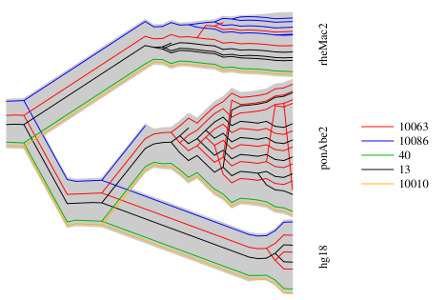
\includegraphics[width=1\textwidth]{images/DUP-tube-tree}}
\caption{Možný vzhľad fylogenetického stromu \cite{Vinar2010}}\label{obr:tree}
\end{figure}
\subsection{Možné zmeny}
Súčasný návrh vizualizácie nezobrazuje všetky informácie zo vstupu. Jedným z údajov, 
ktorý sa stráca je orientácia génu.